\chapter{BIOLINGUISTIQUE ET PSYCHOLINGUISTIQUE : LE LANGAGE DANS LA TÊTE}
\label{chapter-15}
\markright{Biolinguistique et psycholinguistique}
\origpage{470}{456}
\begin{keybox}[Plan du chapitre]
\small\setstretch{1.01}
\textbf{I.\quad LA BIOLINGUISTIQUE}\par
\hspace*{1em}1. Le cerveau : siège du langage\par
\hspace*{2em}\textcircled{\scriptsize 1} Franz Joseph Gall : la phrénologie\par
\hspace*{2em}\textcircled{\scriptsize 2} Paul Broca : l’aire de Broca\par
\hspace*{2em}\textcircled{\scriptsize 3} Carl Wernicke : l’aire de Wernicke\par
\hspace*{2em}\textcircled{\scriptsize 4} Hugues Duffau : remise en cause de l’aire de Broca\par
\hspace*{1em}2. L’évolutionnisme linguistique : la première biolinguistique ?\par
\hspace*{2em}\textcircled{\scriptsize 1} Schleicher : langage et sélection naturelle\par
\hspace*{2em}\textcircled{\scriptsize 2} Primitivisme et progressivisme\par
\hspace*{1em}3. Le programme biolinguistique\par
\hspace*{2em}\textcircled{\scriptsize 1} Le langage, organe mental\par
\hspace*{2em}\textcircled{\scriptsize 2} L’origine du langage : une question à poser\par
\hspace*{3em}1. L’interdit de la Société Linguistique de Paris\par
\hspace*{3em}2. Le « grand bond en avant »\par
\hspace*{3em}3. Ontogénèse et polygénèse\par
\hspace*{2em}\textcircled{\scriptsize 3} Trois facteurs dans l’architecture du langage\par
\medskip
\textbf{II.\quad LA PSYCHOLINGUISTIQUE}\par
\hspace*{1em}1. Psychologie et linguistique : rapprochements et divergences\par
\hspace*{1em}2. Objets d’étude de la psycholinguistique\par
\hspace*{2em}\textcircled{\scriptsize 1} Objets relevant de la linguistique\par
\hspace*{2em}\textcircled{\scriptsize 2} Objets relevant de la psychologie\par
\hspace*{1em}3. Théories de l’acquisition du langage\par
\hspace*{2em}\textcircled{\scriptsize 1} Burrhus Skinner : l’approche béhavioriste\par
\hspace*{2em}\textcircled{\scriptsize 2} Jean Piaget : le constructivisme\par
\hspace*{3em}1. Les paliers d’acquisition\par
\hspace*{3em}2. Assimilation et accommodation\par
\hspace*{2em}\textcircled{\scriptsize 3} Noam Chomsky : le nativisme\par
\hspace*{3em}1. L’hypothèse du LAD (Language acquisition device)\par
\origpage{471}{457}
\hspace*{3em}2. Innéisme et pauvreté du stimulus\par
\hspace*{3em}3. La Grammaire universelle (GU)\par
\hspace*{4em}1) L’héritage de Port Royal\par
\hspace*{4em}2) L’héritage de Descartes\par
\hspace*{2em}\textcircled{\scriptsize 4} Steven Pinker : l’instinct du langage\par
\hspace*{3em}1. The Language Instinct\par
\hspace*{3em}2. Un point de vue évolutionniste\par
\hspace*{2em}\textcircled{\scriptsize 5} L’approche empiriste\par
\hspace*{3em}1. Child Directed Speech et motherese\par
\hspace*{3em}2. La critique de Pinker\par
\hspace*{3em}3. Les travaux de Ochs et Schieffelin\par
\hspace*{4em}1) Chez les Kaluli (Nouvelle-Guinée)\par
\hspace*{4em}2) Chez les Samoans\par
\hspace*{1em}4. La rencontre Piaget-Chomsky\par
\hspace*{2em}\textcircled{\scriptsize 1} Contexte et premiers échanges\par
\hspace*{3em}1. Les arguments en faveur de l’innéisme\par
\hspace*{3em}2. La question de la preuve de l’innéisme\par
\hspace*{2em}\textcircled{\scriptsize 2} L’intervention de Jerry Fodor\par
\hspace*{2em}\textcircled{\scriptsize 3} L’intervention de David Premack\par
\hspace*{2em}\textcircled{\scriptsize 4} L’intervention d’Hilary Putnam\par
\hspace*{2em}\textcircled{\scriptsize 5} Postérité du débat\par
\textbf{III.\quad LE LANGAGE ET SES TROUBLES}\par
\hspace*{1em}1. Dyslexie et dysphasie\par
\hspace*{1em}2. L’aphasie\par
\hspace*{2em}\textcircled{\scriptsize 1} Caractéristiques générales\par
\hspace*{2em}\textcircled{\scriptsize 2} L’aphasie de Broca\par
\hspace*{2em}\textcircled{\scriptsize 3} L’aphasie de Wernicke\par
\hspace*{2em}\textcircled{\scriptsize 4} L’aphasie de conduction\par
\hspace*{1em}3. La dyspraxie\par
\hspace*{2em}\textcircled{\scriptsize 1} Les causes\par
\hspace*{2em}\textcircled{\scriptsize 2} Les symptômes\par
\hspace*{2em}\textcircled{\scriptsize 3} La dyspraxie verbale et « gène de la parole »\par
\textbf{Exercices}\par\textbf{Pour aller plus loin}\par\textbf{Glossaire}
\end{keybox}
\origpage{472}{458}



\section{LA BIOLINGUISTIQUE}
La biolinguistique considère que la langue, sous tous ses aspects (le son, le sens, la structure) est une
composante de la pensée. Dès le 18e siècle, le philosophe David Hume (1711-1776), disait que « La pensée
est une petite agitation du cerveau ». Pour Charles Darwin (1809-1882), les choses sont encore plus claires :
«La pensée est une sécrétion du cerveau ». Près d’un siècle plus tard, au cours de ce que Chomsky appelle
« la décennie du cerveau », les questions sur le rapport entre pensée, langage et cerveau ont fait l’objet de très
nombreuses recherches.
\subsection{Le cerveau : siège du langage}
Même si les choses mentales reposent sur des principes que nous ne comprenons pas encore, la
recherche scientifique permet chaque jour d’en savoir un peu plus sur le cerveau, siège de la pensée,
de la cognition, de la mémoire, des émotions, et aussi du langage. Seul l’homme possède des aires
du cerveau adaptées au langage parlé et à la lecture. Les recherches des pionniers de l’exploration
du cerveau ont montré que le langage résulte d’un ensemble de tâches effectuées dans des régions

\origpage{473}{459}
différentes du cerveau reliées entre elles par un faisceau de fibres. L'un des pionniers de l'exploration

du cerveau est l'allemand Franz Joseph Gall.

\minititle{Franz Joseph Gall : la phrénologie}
Le physiologiste et anatomiste Franz Joseph Gall (1758-1828) a été le fondateur d’une nouvelle
science, la phrénologie qui avait pour but de localiser certaines facultés cérébrales à l’aide de
la forme du crâne. Gall a énoncé sa théorie dans un ouvrage publié en 1810 à Paris et dont le
long titre résume bien le contenu : Anatomie et physiologie du système nerveux en général,
et du cerveau en particulier. avec des observations sur la possibilité de reconnaître plusieurs
dispositions intellectuelles et morales de l'homme et des animaux par la configuration de leur tête.
Selon Gall, le développement du cerveau influe sur la forme du crâne, et une capacité
particulièrement développée (gaieté, causalité, bienveillance, etc.) inscrit sa trace sur le crâne,
comme sur une carte. Cette théorie, souvent raillée et qualifiée de « pseudo-science » a été à l’origine
d’une multitude de travaux et de modèles neuroscientifiques qui incluent tous, bien que chacun à
sa façon, les capacités langagières. Mais ce n'est qu’au 19e siècle que deux scientifiques ont permis
de réelles avancées en localisant le « centre du langage » dans le cerveau.

\minititle{Paul Broca : l'aire de Broca}
Paul Broca (1824-1880) est un médecin, anatomiste et anthropologue français. Sa découverte du
« centre de la parole » dans le cerveau lui a assuré sa place dans l’histoire de la médecine. C’est en
étudiant les cerveaux de patients aphasiques (souffrants de troubles du langage) qu’il a fait cette
découverte. Son premier patient, M. Leborgne, avait été surnommé « Tan », car « tan » était la
seule syllabe qu’il parvenait à prononcer et qu’il répétait sans cesse. Broca a montré que Leborgne
souffrait d’une lésion du lobe frontal gauche, et en a inféré que cette zone était fortement impliquée
dans la production de la parole.
Broca est mort subitement à 56 ans d’un anévrisme cérébral, et son cerveau est conservé au
laboratoire d'Anthropologie du Muséum National d'Histoire Naturelle. Son « centre de la parole »,
connu désormais sous le nom d’aire de Broca, est situé dans le lobe frontal du cerveau. Dans le
classement systématique du neurologue allemand Korbinian Brodmann (1868-1918), qui a
divisé le cortex cérébral de l’homme en 52 aires, l'aire de Broca correspond aux numéros 44 et 45,
comme indiqué dans le schéma ci-dessous :


\begin{figure}[htbp]\centering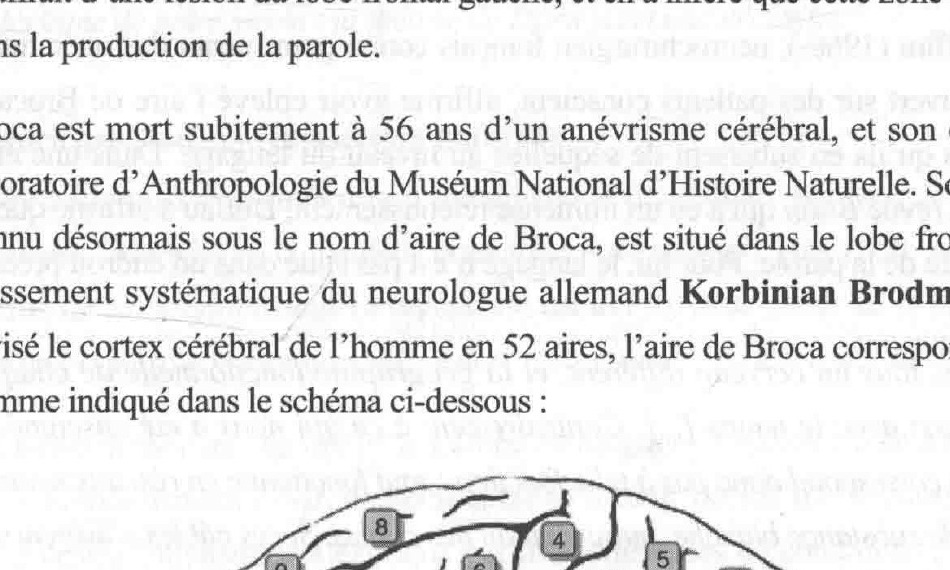
\includegraphics[width=.60\linewidth]{assets/ch15_brodmann_brain.jpg}\caption*{Classement des aires corticales de Brodmann (figure du fond).}\end{figure}
\origpage{474}{460}
\minititle{Carl Wernicke : l'aire de Wernicke}
Neurologue et psychiatre allemand, Karl Wernicke (1848-1905)\ednote{Le plan du chapitre imprime « Carl Wernicke », qui est aussi la forme usuelle du prénom du neurologue ; le corps du texte imprime ici « Karl ». La divergence du fond est conservée.} est, avec Paul Broca, un
précurseur de la recherche sur les localisations cérébrales à travers l'aphasiologie, c’est-à-dire
l'étude des troubles du langage. Wernicke s'est fait connaître en particulier avec ses travaux sur
une zone du cerveau impliquée dans le langage, à laquelle il a laissé son nom.
L'aire de Wernicke est localisée dans le lobe temporal gauche, proche du cortex auditif primaire,
ce qui dans le classement de Brodmann correspond aux numéros 22, 41 et 42. Comme l'aire de
Broca, la fonction de cette aire a été connue par les lésions qui y sont associées : les personnes
ayant une lésion à cet endroit souffrent d’un déficit de compréhension du langage (oral comme
écrit) puisque l'aire de Wernicke est un centre de stockage de la représentation auditive des mots.
L'aire de Broca et l'aire de Wernicke sont reliée par ce qu'on appelle le faisceau arqué, représenté
ci-dessous. Les lésions de ce faisceau engendrent une aphasie dite de conduction, qui sera
présentée en fin de chapitre, avec les autres troubles du langage.
\minititle{Hugues Duffau : remise en cause de l’aire de Broca}
Hugues Duffau (1966-), neurochirurgien français connu pour mener des opérations chirurgicales
à cerveau ouvert sur des patients conscient\ednote{Accord : « patients conscients ». Le fond imprime le singulier « conscient ».}, affirme avoir enlevé l’aire de Broca chez + de 100\ednote{Le signe « + » du fond est employé comme abréviation graphique de « plus » ; en prose suivie : « chez plus de 100 patients ».}
patients sans qu'ils en subissent de séquelles au niveau du langage. Dans une étude publiée en
2014 dans la revue Brain qui a eu un immense retentissement, Duffau a affirmé que l’aire de Broca
n’est pas l'aire de la parole. Pour lui, le langage n’est pas situé dans un endroit précis du cerveau :
\begin{lecture}{Extrait}
Nous avons tous un cerveau différent, et la géographie fonctionnelle de chaque cerveau se modifie aussi avec le temps […]. Contrairement à ce qui nous a été enseigné, telle zone du cerveau ne correspond donc pas à telle fonction : tout fonctionne en réseaux neuronaux, grâce à des fibres de substance blanche, autrement dit des câbles. Si ces câbles s'avèrent similaires d'un individu à l'autre, leurs terminaisons sont en revanche très variables.
\end{lecture}
Pour lui, les observations de Broca étaient justes, mais les généralités qu'il en a tirées sont fausses.
Paul Broca pensait avoir trouvé « la » zone du cerveau qui permet à l’être humain de produire les
mots. Mais il semble que le cerveau ne se découpe pas en zones géographiques qui commandent
chacune une fonction : les dernières découvertes des neurosciences montrent que la parole dépend

\begin{figure}[htbp]\centering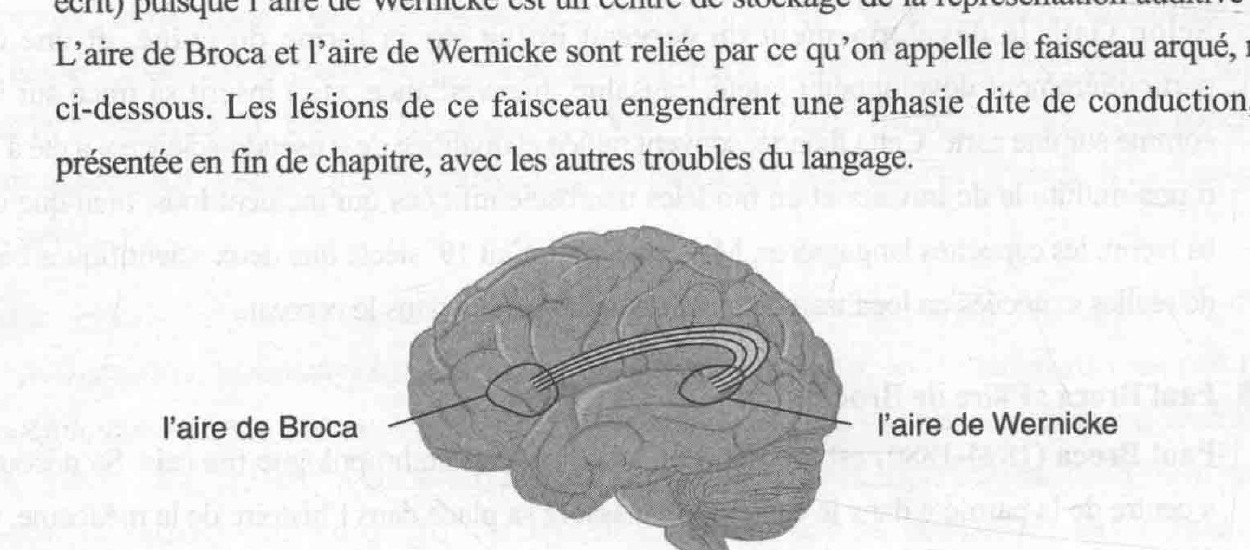
\includegraphics[width=.72\linewidth]{assets/ch15_broca_wernicke.jpg}\caption*{Aires de Broca et de Wernicke et faisceau arqué (figure du fond).}\end{figure}
\origpage{475}{461}
vraisemblablement d'un circuit constitué de fibres reliées entre elles par des nœuds. C'est l'idée
exprimée par Hugues Duffau dans une interview de 2014 au magazine l'Express :
\begin{lecture}{Extrait}
Le fonctionnement du cerveau repose sur des réseaux parallèles capables de se compenser les uns les autres en cas de problème, comme dans le métro parisien, lorsque les voyageurs empruntent des correspondances pour éviter des perturbations sur leur ligne habituelle. On ne parle donc plus de zones, mais de faisceaux. Le nouveau modèle que nous proposons est connexionniste.
\end{lecture}
Les hypothèses « localisationnistes » de Gall, Broca et Wernicke semblent désormais dépassées.
\subsection{L’évolutionnisme linguistique : la première biolinguistique ?}
On sait que, pour Chomsky, la faculté du langage humain est un organe mental dont l'anatomie et
la physiologie sont déterminées par une nécessité biologique, au même titre que celles du cœur et
des poumons. Le langage, objet biologique, constitue un système vivant soumis, comme les autres
systèmes, aux principes de la théorie de l’évolution.
Dans La théorie de Darwin et la science du langage (Die Darwinsche Theorie und die
Sprachwissenschaft, 1868), soit près d'un siècle avant la naissance officielle de la biolinguistique en
1955\ednote{Le passage situe ici une « naissance officielle » en 1955, alors que le même chapitre affirme quelques lignes plus bas que le mot « biolinguistique » serait apparu pour la première fois en 1974. Ces deux datations ne peuvent servir simultanément de repère univoque ; le texte de base est conservé.}, le linguiste allemand August Schleicher (1821-1868) notait déjà :
\begin{lecture}{Extrait}
Des idées semblables à celles que Darwin exprime au sujet des êtres vivants, sont assez généralement admises pour ce qui concerne les organismes linguistiques. […] La théorie de Darwin est ainsi, non pas une manifestation accidentelle, non pas le produit d'une tête fantasque, mais la fille légitime de notre siècle : la théorie de Darwin est une nécessité.
\end{lecture}
\minititle{Schleicher : langage et sélection naturelle}
L'évolutionnisme permet à la biolinguistique de justifier la place de la linguistique parmi les
sciences naturelles et la nature « organique » du langage. Dès 1850, August Schleicher utilise le
terme de Naturorganismus (« organisme naturel »), pour parler de la langue. Selon lui, la langue
est un organisme vivant qui naît, croît et meurt sous l'influence des lois naturelles.
Dans La théorie de Darwin et la science du langage, Schleicher soutient la thèse darwinienne que
le conditionnement environnemental est le facteur décisif de transformation. Selon cette thèse,
la diversité linguistique s'explique par des différences de conditions géographiques, climatiques
et vitales. Dans des conditions équivalentes, la convergence adaptative conduit au contraire les
espèces linguistiques dans la même direction. Schleicher ajoute :

\origpage{476}{462}
\begin{lecture}{Extrait}
Maintenant, ce que Darwin admet pour les espèces animales et végétales, vaut aussi, au moins dans ses traits essentiels, pour les organismes des langues.
\end{lecture}

Il note également que les diverses manières de marcher des divers individus de l’espèce humaine

sont déterminées par la différence dans la constitution des parties du corps qui servent à la marche.

Selon lui, il en va de même pour le langage : bien que la langue ne puisse être appréhendée d’une

manière directe, sa manifestation externe atteste de l'existence d'organes respectifs à cette fonction :

\begin{lecture}{Extrait}
Le langage est la manifestation perceptible à l'oreille, de l'activité d'un ensemble de conditions qui se trouvent réalisées dans la conformation du cerveau et des organes de la parole, ainsi que de leurs nerfs, de leurs os et de leurs muscles.
\end{lecture}

\minititle{Primitivisme contre progressivisme}

À l'époque de Schleicher, les linguistes n’adhéraient pas toujours à l'idéologie du progrès que

l'on retrouvait dans le positivisme d'Auguste Comte (1798-1857) ou dans la philosophie de

Hegel. Les comparatistes Franz Bopp (1791-1867) et Friedrich Schlegel (1772-1829), que

nous avons rencontrés dans le chapitre 5, étaient au contraire des partisans du « primitivisme »

et estimaient que l'état originel des langues représente la perfection, tandis que leurs phases
successives de développement traduisent un déclin. Jacob Grimm (1785-1863) ou Wilhelm von

Humboldt (1767-1835), quant à eux, allaient dans le sens du « progressivisme » en considérant

que les langues flexionnelles sont le sommet et l'aboutissement du développement linguistique.

August Schleicher, en revanche, a adopté une position intermédiaire : essor du développement

des langues isolantes vers les langues flexionnelles par l'intermédiaire des langues agglutinantes,

puis, une fois le point culminant franchi, l'apogée des langues flexionnelles tourne au déclin et à la
dégénérescence.
\subsection{Le programme biolinguistique}
En mai 2004, dans une conférence donnée à Budapest sur le thème « La biolinguistique et la capacité
humaine », Chomsky a ainsi relaté les débuts de cette nouvelle discipline :
\begin{lecture}{Extrait}
La « perspective biolinguistique » a commencé à prendre forme il y a un demi-siècle dans des discussions entre étudiants diplômés qui étaient très influencés par les développements en biologie et en mathématiques au début de l'après-guerre, y compris par les travaux en éthologie dont on venait juste de prendre connaissance aux États-Unis.
\end{lecture}
Divers séminaires et conférences internationales ont suivi, et c'est en 1974 que le mot
«biolinguistique » est apparu pour la première fois\ednote{Cette affirmation est en tension avec la datation de 1955 donnée quelques lignes plus haut dans le même chapitre. La première attestation lexicale du terme demande une vérification historique distincte ; le texte de base est conservé.}.
Le programme biolinguistique est pluridisciplinaire et donc extrêmement vaste : je vais présenter ci-
dessous quelques principes et champs de recherche significatifs mais bien sûr non exhaustifs,

\origpage{477}{463}
\minititle{Le langage, organe mental}
Selon la perspective biolinguistique, il faut traiter le langage comme une propriété biologique et
non comme une faculté intellectuelle faisant l'objet d'un apprentissage, comme les mathématiques
par exemple. La biolinguistique considère la faculté de langage au même titre que les autres
systèmes cognitifs, comme la vision. Pour Chomsky, la faculté de langage est un « organe » mental
dont l'anatomie et la physiologie sont déterminées par une nécessité biologique, au même titre que
celles du cœur et des poumons. Cet organe mental se situe dans le cerveau :
\begin{lecture}{Extrait}
Parmi le grand nombre de phénomènes que l'on pourrait considérer comme liés d'une façon ou d'une autre au langage, l'approche biolinguistique centre son attention sur un composant de la biologie humaine qui entre dans l'usage et l'acquisition du langage, quelle que soit la façon dont on interprète le terme « langage ». Appelons-le la « faculté de langage ». Ce composant est plus ou moins sur un pied d'égalité avec les systèmes visuels des mammifères, la navigation chez les insectes et d'autres choses du même type.
\end{lecture}
\minititle{L'origine du langage : une question à poser}
L'établissement d’un rapport entre la linguistique et la biologie a initié un renouveau d'intérêt sur
la question de l’origine et du développement du langage humain.
\minititle{1. L'interdit de la Société Linguistique de Paris}
Dès les toutes premières lignes de notre livre, nous avons vu que la Société de Linguistique de
Paris avait, en 1866, interdit les travaux sur l'origine du langage. Nous avons aussi vu que pour
Saussure la question de l’origine du langage n'est même pas une question à poser. On voit ci-
dessous le point de vue identique d’un linguiste français oublié, Victor Henry (1850-1907) :
\begin{lecture}{Extrait}
Que le linguiste doive s'interdire toute recherche sur l'origine du langage, c'est un point qui semble définitivement acquis, tout au moins parmi les linguistes, si paradoxale qu'en soit la première apparence : l'origine du langage n'est pas, a priori, un problème linguistique, puisque la linguistique ne se propose pour objet que des langues formées, dans leur état actuel, historique ou préhistorique, et qu'il ne lui est donné que de constater l'évolution, jamais la naissance du langage.
\end{lecture}
Cet interdit de la Société de Linguistique de Paris a finalement été levé au début des années 1980,
et les années 1990 ont vu une explosion des recherches sur la question de l'origine de langage. Ces
réflexions ont été étayées non seulement par des arguments provenant de l'étude de l'acquisition
du langage par les enfants, mais aussi de l'étude des créoles qui permettent d'assister en quelque
sorte à la naissance de nouvelles langues « en direct »\origfoot{1}{Le linguiste américain Derek Bickerton a publié sur ces questions des ouvrages remarqués : \textit{Lingua ex Machina: Reconciling Darwin and Chomsky with the Human Brain} (2000), et, plus récemment, \textit{La Langue d’Adam} (2010).}.

\origpage{478}{464}
\minititle{2. Le « grand bond en avant »}
De nos jours, de nombreux scientifiques sont d'accord avec le paléoanthropologue américain
Tan Tattersall pour qui l'invention du langage a été le stimulus déclencheur de l'apparition des
capacités cognitives humaines. C’est ce que le biologiste Jared Diamond (1937-) appelle le
«grand bond en avant » : c’est un événement génétique touchant le cerveau qui a permis l'apparition
du langage moderne, avec une riche syntaxe fournissant une multitude de modes d'expression
de la pensée. Dans cette optique, le langage est vu comme un pré-requis pour le développement
social et c'est l'apparition du langage qui a permis des changements brusques de comportement,
comme le départ d'Afrique (hypothèse de la monogénèse présentée dans notre premier chapitre)
attesté par des données archéologiques. Avant Diamond, le biologiste darwiniste allemand Ernst
Haeckel (1834-1919) avait présenté une idée très proche dans son Histoire de la création des êtres
organisés d'après les lois naturelles (1874). À propos du rôle du langage dans le développement
du cerveau en connexion avec d'autres aptitudes cognitives, il écrivait :
\begin{lecture}{Extrait}
Rien n'a dû ennoblir et transformer les facultés et le cerveau de l'homme autant que l'acquisition du langage. La différenciation plus complète du cerveau, son perfectionnement et celui de ses plus nobles fonctions, c'est-à-dire des facultés intellectuelles, marchèrent de pair et en s’influençant réciproquement, avec leur manifestation parlée.
\end{lecture}
Notez que chez Haeckel, la faculté du langage est présentée en interaction constante avec d’autres
domaines cognitifs, idée largement admise de nos jours.
\minititle{Trois facteurs dans l'architecture du langage}
En supposant que la faculté de langage a les propriétés générales d'autres systèmes biologiques et
cognitifs, Chomsky identifie trois facteurs qui entrent dans la «croissance » (terme préféré à celui
d'apprentissage) du langage chez l'individu :
\noindent\textcolor{BellaTeal}{$\diamond$}\enspace d'abord, l'héritage génétique, uniforme pour l'espèce humaine, et qui ancre la linguistique\par
dans la biologie ;
\noindent\textcolor{BellaTeal}{$\diamond$}\enspace l'expérience, qui conduit à la variation à l'intérieur d’une gamme relativement étroite, comme\par
en biologie, où une même espèce ne contient pas d'instances identiques ;
\noindent\textcolor{BellaTeal}{$\diamond$}\enspace enfin, des principes qui ne sont pas spécifiques à la faculté de langage. Ce dernier point est\par
important, car il indique les propriétés du langage peuvent être spécifiques au langage, mais
aussi intervenir dans d’autres domaines cognitifs.
Cette activité cognitive, dont la capacité générative dans le Programme Minimaliste réside en une
opération binaire récursive, offre par sa simplicité une modélisation compatible avec l'émergence
du langage. Quant à l'hypothèse selon laquelle le langage a émergé par un changement dans
le cerveau humain, elle se distingue nettement de l'approche évolutionniste, mais le fait que le
langage soit une innovation récente dans l'évolution des espèces rend l'hypothèse évolutionniste

\origpage{479}{465}
peu probable. Quoi qu'il en soit, l’entreprise biolinguistique a le mérite d'avoir ouvert de nouvelles
voies de recherche et a permis, comme l’a souligné Chomsky lui-même, d'aller au-delà de
l'adéquation explicative et de lier les propriétés formelles du langage à son origine biologique.
\section{LA PSYCHOLINGUISTIQUE}
Le terme de psycholinguistique a été créé en 1951\ednote{Formulation historiquement contestable : le séminaire de Cornell de 1951 a joué un rôle institutionnel majeur, mais le terme anglais psycholinguistics est attesté auparavant. Il vaut mieux parler ici d’institutionnalisation du champ que de création certaine du mot.} lors d’un séminaire d'été de l’Université de Cornell, aux
États-Unis, auquel ont participé des linguistes et psychologues comme Charles Osgood (1916-1991) et
Thomas Sebeok (1920-2001). Un autre séminaire, organisé en 1953, a été à l’origine de la publication d’un
livre fondateur, fruit de la collaboration de Charles Osgood et Thomas Sebeok, et intitulé Psycholinguistic.\ednote{Le titre de l’ouvrage issu du programme Osgood-Sebeok est généralement donné au pluriel : « Psycholinguistics: A Survey of Theory and Research Problems » (1954). Le singulier imprimé dans le fond paraît être une coquille.}
Cet ouvrage comporte un vaste programme de recherches visant à faire la synthèse entre la psychologie
de l'apprentissage, la théorie de l'information tout juste créée par Claude Shannon (1916-2001), et la
linguistique.
\subsection{Psychologie et linguistique : rapprochements et divergences}
Les premières recherches en psycholinguistique ont largement été influencées par la théorie de
l'information de Claude Shannon, selon laquelle la langue est un code et le comportement verbal une
activité d'encodage et de décodage. La collaboration entre psychologie et linguistique a été fructueuse
initialement : même si leur objet d'étude est différent, elles cherchent toutes les deux à étudier la nature
du langage et le fonctionnement de celui-ci dans le cerveau. De ce point de vue, les informations
linguistiques permettent de mieux comprendre ce qui se passe dans le cerveau.
La psycholinguistique s'intéresse à la réalité psychologique des théories linguistiques. Elle part d'un
point de vue formel sur la langue (celui de la linguistique), pour tenter de voir de quelle façon le
fonctionnement linguistique est inscrit dans un fonctionnement psychologique. Les années 60 ont été
marquées par l'attention que les psycholinguistes ont accordée à la grammaire générative de Chomsky
pour tenter d’en démontrer la réalité psychologique : c’est ce qu’on appelle la psycholinguistique
chomskyenne. Mais à partir des années 70, la psycholinguistique a réagi contre son assujettissement
antérieur à la linguistique générative et s’est intégrée plus étroitement à la psychologie cognitive,
discipline qui étudie les processus mentaux (fonctionnement du système) et les composantes
(architecture du système) impliqués dans le traitement de l'information. Avec les progrès récents
de la psychologie cognitive et l'émergence de modèles généraux de fonctionnement cognitif, les
psychologues cognitifs ont été conduits à faire le chemin inverse, c'est-à-dire tester la validité des
règles générales du fonctionnement cognitif à travers les cas particuliers des activités du langage.
\subsection{Objets d’étude de la psycholinguistique}
En psycholinguistique, on distingue traditionnellement, et c'est bien compréhensible, les objets qui
relèvent de la linguistique de ceux qui relèvent de la psychologie.
\minititle{Objets relevant de la linguistique}
\noindent\textcolor{BellaTeal}{$\diamond$}\enspace L'acquisition du langage. C'est le domaine de recherche qui vise à décrire et comprendre\par

\origpage{480}{466}
comment l'enfant acquiert le langage à partir du milieu qui l'entoure.
La perception du langage. Il s’agit de l'étude des processus qui transforment un signal externe
en une représentation cognitive interne abstraite.
\noindent\textcolor{BellaTeal}{$\diamond$}\enspace La compréhension du langage. Il faut distinguer ici la compréhension du langage oral et\par
écrit, car la capacité à interpréter des textes se fait au moyen de connaissances linguistiques
mais aussi extralinguistiques. Ce domaine s'intéresse aussi aux inférences que le destinataire
va émettre, et qui portent sur les intentions du locuteur : la dimension pragmatique est très
importante ici.
La production discursive : il s’agit ici d'étudier les processus mentaux et physiques nécessaires
à la production du langage. j
\minititle{Objets relevant de la psychologie}
Aux quatre objets ci-dessus, on ajoute généralement les objets d'étude suivants :
\noindent\textcolor{BellaTeal}{$\diamond$}\enspace Langage et fonctionnement cérébral : ce domaine d'étude vise à localiser les processus\par
cognitifs au niveau cérébral en utilisant des techniques évoquées plus haut, et notamment
l'imagerie cérébrale (IRM). On cherche aussi à identifier les modules du cerveau impliqués
dans le traitement et la production du langage.
\noindent\textcolor{BellaTeal}{$\diamond$}\enspace Langage et émotions : ce domaine d'étude cherche à déterminer à quel moment le système\par
affectif intervient dans le traitement du langage. Notre vie quotidienne nous rappelle que
notre état émotionnel peut en effet avoir des conséquences sur la cognition et le traitement du
langage.
Il existe bien sûr bien d’autres domaines de recherche, mais, comme dans le cas de la
biolinguistique un peu plus haut, seuls les plus caractéristiques ont été évoqués ici.
\subsection{Théories de l’acquisition du langage}
La méthode par laquelle les enfants développent les capacités langagières est universelle : tous les
enfants du monde entier, sauf dans les cas de troubles du langage que nous présenterons un peu plus
bas, apprennent à parler. Cependant, il reste à savoir comment le langage est acquis. Pour tenter de
répondre cette question, trois approches ont été avancées\ednote{Le fond annonce « trois approches », puis en énumère quatre : béhavioriste, constructiviste, nativiste et empiriste.}
une approche béhavioriste, héritée du « Verbal Behavior » de Skinner, et basée sur le renforcement
opérant ;
une approche constructiviste, qui met en avant l’activité du sujet pour se construire une
représentation de la réalité en la « reconstruisant » ;
\noindent\textcolor{BellaTeal}{$\diamond$}\enspace une approche nativiste selon laquelle certains principes de syntaxe sont innés et transmis par le\par
génome humain ;

\origpage{481}{467}
une approche empiriste selon laquelle les enfants apprennent toutes les règles syntaxiques à partir
des données linguistiques tirées de leur environnement.
\minititle{Burrhus Skinner : l'approche béhavioriste}
Sans vouloir répéter ce que nous avons dit dans le chapitre précédent, il est important d’une part
de rappeler que le behaviorisme a dominé toute la psychologie jusqu'à la fin des années 1950,
et d'autre part de préciser qu'il a grandement influencé la psycholinguistique née, on le sait, à la
même époque : on peut dire que la première génération de psycholinguistes est née de la rencontre
de linguistes et d'adeptes d'un behaviorisme modéré.
En se limitant à ce qui peut être observé, les béhavioristes rejettent toute référence à l’âme, à
l'esprit ou à la conscience et refusent de considérer les états mentaux et de façon générale le
fonctionnement intellectuel de l'humain comme des objets d'observation : tout ce qui se situe à
l'intérieur de la « boîte noire » est inaccessible à toute étude objective.
Pour Skinner, on l'a vu, le langage est considéré comme un comportement et analysé comme tel.
Selon lui, les enfants apprennent donc à parler comme ils apprennent d'autres comportements,
c'est-à-dire par un renforcement opérant résultant d’un apprentissage social. Le langage est appris
par réaction à des stimuli et par renforcement des réponses correctes selon le schéma : stimulus →
réponse → correction.
\minititle{Jean Piaget : le constructivisme}
Le constructivisme est une théorie de l'apprentissage développée dès 1923 par le psychologue
suisse Jean Piaget (1896-1980) en réaction contre le béhaviorisme qui, d'après lui, limitait trop
l'apprentissage à l'association stimulus-réponse L'approche constructiviste met en avant l’activité
du sujet pour se construire une représentation de la réalité qui l'entoure, et suppose que les
connaissances de chaque sujet ne sont pas une simple copie ou une imitation de la réalité, mais une
reconstruction de celle-ci. Pour Jean Piaget, l'intelligence n’est pas innée mais se construit, et le
développement intellectuel de l'enfant se construit selon une série de paliers hiérarchisés.
\minititle{1. Les paliers d'acquisition}
C'est en 1936, dans un ouvrage intitulé Les origines de l'intelligence chez l'enfant que Piaget a
présenté sa théorie des paliers. Cette théorie très influente, révisée ultérieurement par Piaget lui-
même, a fait l’objet de nombreuses études et a beaucoup influencé la recherche en psychologie
du développement durant la seconde moitié du 20e siècle. Voici les cinq stades d'acquisition selon
Piaget\ednote{L’énumération qui suit comporte quatre stades : sensorimoteur, préopératoire, opératoire concret et opératoire formel. « cinq » est donc incohérent avec la liste donnée dans le fond.} :
Le stade sensorimoteur se met en place de la naissance jusqu'à 2 ans. Le bébé utilise les sens
et la motricité pour découvrir le monde qui l'entoure.
\noindent\textcolor{BellaTeal}{$\diamond$}\enspace Le stade préopératoire marque l'apparition du langage. Après ses 2 ans et aux alentours de 5\par
ou 6 ans, c'est à ce moment-là que se développent l'imitation, la représentation et la réalisation
d'actes fictifs. Lors d'un jeu, par exemple, un tronc d'arbre devient une table, et un objet se
\origpage{482}{468}
substitue à un autre.
\noindent\textcolor{BellaTeal}{$\diamond$}\enspace Le stade opératoire concret. L'enfant, entre 7 et 12 ans, raisonne concrètement, peut classer,\par
grouper. Il se socialise, prend en compte ce que disent les autres.
\noindent\textcolor{BellaTeal}{$\diamond$}\enspace Le stade opératoire formel est caractérisé par l’abstraction et la mentalisation. À partir de 12\par
ans, la pensée devient hypothético-déductive : l'enfant peut combiner des idées, raisonner
par des hypothèses, et faire des déductions. Les opérations portent sur des propositions
verbales, donc des objets linguistiques. Le raisonnement, quant à lui, porte sur des propositions
abstraites et non sur des actions en lien avec le réel.
Le développement des capacités langagières, qui nous concerne plus directement, se fait, on
l'a vu, et pour l'essentiel, au cours de la deuxième phase : celle de l'intelligence préopératoire.
C'est au cours de cette période qu'émerge chez l'enfant une pensée symbolique se manifestant
de deux façons. L'une, selon Piaget, est l'apparition du langage articulé. L'autre est une conduite
caractéristique de la pensée symbolique : le jeu symbolique, lorsque l'enfant joue à faire « comme
si ». Puis, au contact des personnes de son entourage (famille, école, etc.), ce langage balbutiant va
peu à peu se développer, se ramifier, s'affiner, tant du point de vue de la richesse lexicale que de la
maîtrise de la syntaxe. Piaget insiste sur le fait qu'il s'agit d’une construction, d’un apprentissage.
\minititle{2. Assimilation et accommodation}
À chacun des paliers présentés ci-dessus, l'enfant va se construire, intégrer le réel, et tout
cela dépend du milieu dans lequel il se trouve. Normalement, l'enfant acquiert la capacité de
communication verbale entre 18 et 25 mois, si le milieu lui est favorable. Cette intégration du réel
se fait à partir de deux opérations : l'assimilation et l’accommodation.
Piaget définit l'assimilation comme le processus qui transforme le milieu pour l'adapter aux
connaissances de l'individu. Connaître ne consiste pas à copier le réel mais à agir sur lui :
c’est donc par un processus d'adaptation que l'individu intègre de nouvelles informations ou
expériences, L'assimilation va de l'objet vers le sujet, et s'oppose à l'accommodation qui, allant du
sujet vers l'objet, permet l'adaptation d'un individu à son milieu.
C'est dans La construction du réel chez l'enfant (1937) et Biologie et connaissance (1967) que
sont développés les concepts d'assimilation et d'accommodation, définis comme suit
\begin{lecture}{Extrait}
Nous prenons le terme d'assimilation au sens d'une intégration à des structures préalables […] qui peuvent demeurées inchangées ou sont plus ou moins modifiées par cette intégration même, mais sans discontinuité avec l'état précédent, c'est-à-dire sans être détruites et en s'accommodant simplement à la nouvelle situation. […] Nous appellerons accommodation […] toute modification des schèmes d'assimilation sous l'influence de situations extérieures (milieu) auxquelles ils s'appliquent. Mais de même qu'il n'y a pas d'assimilation sans accommodation (antérieures ou actuelles), de même il n'y a pas d'accommodation sans assimilation.
\end{lecture}

\origpage{483}{469}
\minititle{Noam Chomsky : le nativisme}
En psychologie, le débat entre inné et acquis oppose les défenseurs de l'innéisme à ceux qui
privilégient une approche dans laquelle l’environnement joue un rôle plus prépondérant sur
l'acquisition d’un comportement donné. Pour Piaget, l'acquisition du langage se fait par étapes,
en interagissant avec le monde extérieur : elle relève donc essentiellement de l'acquis et s'intègre
dans le cadre plus général du développement de l'intelligence.
La thèse opposée, celle de l’innéisme, qui constitue le cœur de la révolution chomskienne, est elle
aussi une réaction contre Skinner, et certains des arguments nativistes qui seront repris ensuite
par Chomsky se trouvaient déjà dans son compte rendu virulent de Verbal Behavior (1959). Pour
Chomsky, les règles de grammaire que nous apprenons à l'école ne constituent que la partie
émergée d’un gigantesque iceberg : ce qui est enseigné à l’école est ce qui varie d’une langue à
l'autre, Mais il existe d’autres règles sous-jacentes beaucoup plus générales, voire universelles,
que nous utilisons sans les avoir jamais apprises, et ce dès le plus jeune âge. Ces règles tacites que
nous maîtrisons intuitivement constituent aux yeux de Chomsky et des linguistes de sa mouvance
la meilleure preuve que la faculté de langage est innée.
\minititle{1. L'hypothèse du LAD (Language acquisition device)}
Avec sa théorie de la grammaire générative, Chomsky soutient donc l'idée très novatrice à
l'époque qu'il est impossible pour les enfants d'apprendre le langage uniquement à partir de
leur environnement. Selon lui, l'acquisition du langage serait plutôt assimilable à l'exécution
d'un programme informatique implanté dans notre cerveau dès notre naissance. Dans Syntactic
Structures (1957), il défend l’idée que les enfants possèdent dès leur naissance un dispositif
d'apprentissage du langage (language acquisition device), et c'est parce qu'ils possèdent ce LAD
que les enfants sont capables d'apprendre si rapidement et sans efforts le langage, et cela malgré
l'information incomplète en provenance de l'environnement, Chomsky suppose que ce LAD est
une aire du cerveau\ednote{Le LAD chomskyen est un dispositif théorique d’acquisition du langage, non le nom d’une aire cérébrale anatomiquement localisée. L’identification à « une aire du cerveau » simplifie abusivement le concept.} qui contient un ensemble de règles universelles pour tous les langages : c'est
ce qu'il appelle la Grammaire Universelle (universal grammar), sur laquelle je vais revenir un
peu plus bas. Quant à ce programme spécialisé implanté dans notre cerveau, Chomsky l’a nommé
« module du langage » et a fourni de nombreux arguments en faveur pour prouver son existence.
\minititle{2. Innéisme et pauvreté du stimulus}
Pour justifier la thèse de l'innéisme et faire face à leurs détracteurs, Chomsky et ses successeurs ont
constitué un dispositif argumentatif, dont on voit ci-dessous des arguments les plus fréquemment
mis en avant :
\noindent\textcolor{BellaTeal}{$\diamond$}\enspace La vitesse de l'apprentissage. L'apprentissage de la langue maternelle est remarquablement\par
rapide, étant donné la complexité des langues.
\noindent\textcolor{BellaTeal}{$\diamond$}\enspace L'inéluctabilité de l'apprentissage. Les enfants réussissent toujours à apprendre leur langue.\par
\noindent\textcolor{BellaTeal}{$\diamond$}\enspace La productivité. Le nombre d’énoncés produits (performance) ou compris (competence)\par

\origpage{484}{470}
est potentiellement infini, L'apprentissage ne peut donc reposer sur la simple limitation
des productions adultes, mais repose sur une capacité créatrice : les enfants ne sont pas des
imitateurs serviles.

\noindent\textcolor{BellaTeal}{$\diamond$}\enspace La sous-exposition. Connu aussi sous le nom de pauvreté du stimulus (poverty of stimulus), il\par
s'agit de l'argument le plus souvent avancé pour prouver le caractère inné de l'apprentissage
du langage chez les enfants. Selon Chomsky, les données linguistiques primaires (primary
linguistic data) dont l'enfant dispose sont pauvres, fragmentaires, insuffisantes. Dans Aspects
of the Theory of Syntax (1965), exprimait l’idée suivante\ednote{La phrase du fond est syntaxiquement incomplète : le sujet du verbe « exprimait » manque. Une rédaction attendue serait, par exemple, « Dans Aspects of the Theory of Syntax (1965), Chomsky exprimait l’idée suivante ».} :

\begin{lecture}{Extrait}
Much of the actual speech observed by children consists of fragments and deviant expressions of various sorts.
\end{lecture}
Et en effet, parmi les données qui constituent de l’environnement linguistique de l'enfant, certaines
formes sont agrammaticales, incomplètes, ambiguës, insuffisamment fréquentes, etc. Et pourtant,
les enfants, confrontés à ces données partielles et défectueuses, n'en apprennent pas moins leur
langue. D'autre part, certains enfants sous-exposés à une langue finissent par en construire une :
c'est le cas des enfants exposés à des pidgins, ou des enfants sourds élevés en milieu entendant.
Cette ligne d’argumentation invalide la théorie de l'empirisme, basée sur le « stimulus »
linguistique, et que nous présenterons un peu plus bas. Mais revenons d’abord.

\minititle{3. La Grammaire universelle (GU)}

Dans sa Grammaire Universelle (GU), Chomsky défend la thèse d’une grammaire universelle et

innée. Mais l'idée de grammaire universelle n’est pas entièrement nouvelle : on en trouvait déjà les

prémisses au 17e siècle chez Port Royal et dans la philosophie cartésienne.
\minititle{1) L'héritage de Port Royal}
Dans son ouvrage Le langage et la pensée (1968), Chomsky revendique l'héritage de Port
Royal et fait l'hypothèse de ce qu’il appelle des « universels linguistiques », c'est-à-dire des
Structures communes à toutes les langues, inscrites dans l’esprit humain : tout se passe comme
si nous étions « prédisposés » à apprendre une grammaire, et comme si cette connaissance
était par conséquent déjà inscrite dans la structure de la faculté du langage. La grammaire
universelle est, pour Chomsky, l'hypothèse la plus explicative de l'apprentissage de la langue :
malgré des différences superficielles, la structure des langues est universelle puisque basée sur
l'esprit humain, le logos, lui-même universel.
\minititle{2) L'héritage de Descartes}
L'emprunt de Chomsky à la philosophie de Descartes, les « idées innées » évoquées dans les
Méditations Métaphysiques : « Nous apprenons à connaître les vérités innées par la force de
notre intelligence, sans aucune expérience sensorielle. »


\origpage{485}{471}
L'innéisme de Chomsky s'inscrit donc dans une position philosophique qui remonte à Platon.
Signe de l'influence de la pensée cartésienne sur Chomsky, ce dernier a publié en 1966 un
ouvrage intitulé Cartesian Linguistics. A Chapter in the history of rationalist thought, traduit
en français en 1969 sous le titre La linguistique cartésienne. Un chapitre de l'histoire de la
pensée rationaliste.
\minititle{Steven Pinker : l'instinct du langage}
Steven Pinker (1954-), est un psychologue cognitiviste canadien. Auteur à succès d'ouvrages
de vulgarisation, il est connu pour son plaidoyer en faveur de la psychologie évolutionniste et la
théorie computationnelle de l'esprit (qui sera présentée dans notre dernier chapitre).
\minititle{1. The Language Instinct}
Dans The Language Instinct (1994), Pinker présente la langue comme un instinct, un produit
de l'adaptation biologique façonné par la sélection naturelle. Il y défend aussi la thèse nativiste
chomskienne selon laquelle les humains naissent avec une capacité innée pour le langage (All
infants come into the world with linguistic skills). Autre point d'accord avec Chomsky, cette faculté
innée qui repose sur des capacités spécifiques est dissociées de la cognition ou de l'intelligence «
générale » : c'est la thèse de la modularité du langage. Quant à la grammaire universelle, Pinker
affirme lui aussi qu'elle est implémentée dans le cerveau humain :
\begin{lecture}{The Language Instinct}
Surprisingly, though practice is important in training for the gymnastics of speaking, it may be superfluous in learning grammar:
\end{lecture}
Selon lui, les structures nécessaires à l'apprentissage du langage n'existent qu'à un certain âge
et sont évacuées ensuite pour alléger le fonctionnement du cerveau : il y aurait donc une période
critique dans l'apprentissage du langage, et cela expliquerait d'une part la rapidité avec laquelle les
enfants acquièrent leur langue maternelle, et d'autre part la difficulté de l'apprentissage à un âge
tardif des langues.
\minititle{2. Un point de vue évolutionniste}
Pinker, on l’a vu, appartient au courant de la psychologie évolutionniste : il s'éloigne de Chomsky
en utilisant la théorie de l'évolution qui peut expliquer cet instinct du langage. Selon lui, le
langage, aptitude unique aux humains, est un produit de l'évolution né de la nécessité de résoudre
des problèmes de communication au sein des groupes chez nos ancêtres chasseurs et pêcheurs.
Il compare aussi le langage à d’autres exemples d'adaptations chez d'autres espèces, comme le
tissage de toile de l’araignée ou la construction de barrages chez le castor. Il est intéressant de
noter que si Pinker considère le langage comme un instinct, c'est pour le distinguer des inventions
humaines, comme la métallurgie où même l'écriture. Alors que certaines cultures seulement
possèdent ces technologies, toutes les cultures sans exception possèdent le langage.
\origpage{486}{472}
\minititle{L’approche empiriste}

En opposition à Chomsky et à son argument de la pauvreté du stimulus, la théorie empiriste

suggère que les données linguistiques primaires (DLP) dont disposent les enfants sont suffisantes

et que les processus cérébraux généraux sont suffisants pour l’acquisition du langage. Par

conséquent, l'hypothèse de l'existence d'un LAD n'est pas nécessaire : c’est activement, et au

travers d'interactions avec son environnement, que l'enfant apprend le langage.

\minititle{1. Child Directed Speech et motherese}

Selon la théorie empiriste, pour qu’un enfant apprenne le langage, le parent ou toute personne qui

s'en occupe adopte une façon de communiquer appropriée : c'est le motherese, appelé aussi infant-

directed speech (IDS) ou child-directed speech (CDS). Ce « mamanais » (langage des mères) se

caractérise par un vocabulaire simplifié, un rythme de parole plus lent, des répétitions fréquentes et

une voix chantante et aiguë. C'est d'ailleurs ce que Pinker indique dans son Instinct du langage :
\begin{lecture}{The Language Instinct}
Motherese has interpretable melodies: a rise-and-fall contour for approving, a set of sharp, staccato bursts for prohibiting, a rise pattern for directing attention, and smooth, low legato murmurs for comforting. The psychologist Anne Fernald has shown that these patterns are very widespread across language communities, and may be universal. The melodies attract the child’s attention, mark the sounds as speech as opposed to stomach growlings or other noises, distinguish statements, questions, and imperatives, delineate major sentence boundaries, and highlight new words. When given a choice, babies prefer to listen to Motherese than to speech intended for adults.
\end{lecture}

Malgré la simplicité du mamanais, qui pourrait aller dans le sens de l'argument de la pauvreté du

stimulus de Chomsky, il faut noter que les parents et autres adultes qui interagissent avec l'enfant

utilisent des phrases plus longues que celles de l'enfant et à reformuler ce qu'il dit. Par exemple, si

jeune enfant qui dit « chien méchant », l'adulte a tendance à répondre « Oui, le chien est méchant ».

Toutefois, le mamanais n’est pas un phénomène universel : nous allons le voir, il existe des

cultures dans lesquelles les adultes parlent aux enfants comme aux adultes, et d'autres cultures où

ils ne s'adressent pas à eux. Et pourtant ces enfants apprennent néanmoins le langage à un rythme

normal. Pour Pinker, cela permet de remettre en cause l'utilité du mamanais.

\minititle{2. La critique de Pinker}

Dans The Language Instinct, Pinker explique l'idée contre-intuitive que le mamanais n'est pas aussi

simple qu'il y paraît :
\begin{lecture}{The Language Instinct}
Motherese is not grammatically simple. That impression is an illusion: grammar is so instinctive that we do not appreciate which constructions are complex until we try to work out the rules behind them. Motherese is riddled with questions containing who, what, and where, which are among the most complicated constructions in English.
\end{lecture}


\origpage{487}{473}
Mais surtout, reprenant l'argument des cultures dans lesquelles les adultes ne s'adressent pas aux
enfants, il considère que le mamanais est superflu :
\begin{lecture}{The Language Instinct}
Motherese is not an indispensable curriculum of Language-Made-Simple lessons. In some cultures, parents do not talk to their children until the children are capable of keeping up their end of the conversation (though other children might talk to them).
\end{lecture}
Ici, Pinker fait référence de façon implicite aux travaux des ethnologues américaines Elinor Ochs
et Bambi Schieffelin.
\minititle{3. Les travaux de Ochs et Schieffelin}
Représentantes de la linguistique anthropologique contemporaine, Elinor Ochs (1944-) et Bambi
Schieffelin (1945-) ont comparé les modes d'acquisition du langage dans trois cultures : chez
la classe moyenne américaine, chez les habitants des Îles Samoa, et chez les Kaluli (une ethnie
de la Nouvelle Guinée Papouasie). La culture américaine a ceci de remarquable, comparée aux
deux autres, que les adultes adaptent leur façon de parler aux enfants, et s'abaissent au niveau des
enfants (self-lowering strategy) qu'ils considèrent comme des interlocuteurs compétents. Ce n'est
pas le cas des Kaluli et des Samoans.
\minititle{1) Chez les Kaluli (Nouvelle-Guinée)}
Chez les Kaluli, Bambi Schieffelin a observé que les mamans ne s'adressent que très rarement
à leurs enfants, considérés comme des interlocuteurs non compétents :
\begin{lecture}{Ochs et Schieffelin}
Kaluli mothers, given their belief that infants “have no understanding” never treat their infants as partners (speaker/addressee) in dyadic communicative interactions. Although they greet their infants by name and expressive vocalizations, they rarely address other utterances to them.
\end{lecture}
Toutefois, Ochs et Schieffelin n'en déduisent pas que les enfants vivent dans un environnement
linguistiquement pauvre, ni qu’ils ne sont pas exposés qu'aux DLP produites par d’autres
enfants. Selon elles, c'est tout le contraire :
\begin{lecture}{Ochs et Schieffelin}
However, this does not mean that children grow up in an impoverished verbal environment and do not learn how to speak. Quite the opposite is true. The verbal environment of the infant is rich and varied, and from the very beginning the infant is surrounded by adults and older children who spend a great deal of time talking to one another. Furthermore, as the infant develops and begins to crawl and engage in play activities and other independent actions, these actions are frequently referred to, described, and commented upon by members of the household, especially older children, to each other:
\end{lecture}

\origpage{488}{474}
\minititle{2) Chez les Samoans}
Dans Talking to children in Western Samoa (1982), Elinor Ochs a montré que l’environnement
linguistique chez les Samoans est exempt des simplifications du mamanais : les adultes
s'adressent aux enfants comme à d'autres adultes. Cette attitude s'explique par le statut social
de l'enfant : pour les Samoans, il ne convient pas qu'un supérieur adapte son comportement
à un individu subalterne. Or, l'enfant est un subalterne, et en tant que tel, il n’est pas un
interlocuteur à part entière. La situation de communication est donc triangulaire : le supérieur
délègue le soin de s'occuper de l'enfant à un subalterne et n’échange pas directement avec
l'enfant. Comme chez les Kaluli, les adultes ne tentent pas non plus d'interpréter les paroles
de l'enfant ni de conjecturer ses intentions : c'est l'enfant qui est amené lui-même à les
clarifier. Et comme pour les Kaluli, Ochs et Schieffelin ne parlent nullement d'environnement
appauvri : même si les adultes ne dialoguent pas avec les enfants, ces derniers sont en situation
overhearers, c'est-à-dire en position d'écoute de conversations entre adultes qui ne leur sont
pas destinées directement.
\subsection{La rencontre Piaget-Chomsky}
En 1975, Piaget et Chomsky exposeront leurs thèses respectives dans un débat devenu célèbre. C’est
en France, à la Fondation Royaumont, co-organisatrice un an plus tôt de la rencontre de Dedham, que
Jean Piaget et Noam Chomsky ont confronté leur théorie de l'acquisition du langage dans un débat
devenu depuis historique.
\minititle{Contexte et premiers échanges}
Si un très grand nombre de chercheurs (psychologues, linguistes, philosophes, neurologues, etc.)
ont participé au débat, l'enjeu était de confronter deux conceptions opposées de la genèse de la
pensée et du langage : l'innéisme de Chomsky et le constructivisme de Piaget. Piaget a ouvert la
discussion par un texte résumant sa théorie et précisant que la pensée ne fonctionne pas par un
simple enregistrement passif des données de l'environnement, comme le supposent les empiristes.
Il a ensuite fait un pas en direction de Chomsky
Je suis d'accord sur le principal apport de Chomsky à la psychologie, le langage est un produit
de l'intelligence ou de la raison et non pas d'un apprentissage au sens béhavioriste du terme.
Je suis ensuite d'accord avec lui sur le fait que cette origine rationnelle du langage suppose
l'existence d'un noyau fixe nécessaire à l'élaboration de toutes les langues […]. Je pense qu'il y
a accord sur l'essentiel, et je ne vois aucun conflit important entre la linguistique de Chomsky et
ma propre psychologie
Cela dit, pour saisir le réel, il faut à l'enfant des cadres mentaux, et ces cadres mentaux, pour
Piaget, ne sont pas innés. Chomsky a reconnu qu'il existe trois conceptions de l'acquisition du
langage : l’empirisme, l’innéisme et le constructivisme. Piaget se définissant lui-même comme
constructiviste, Chomsky s’est rangé sans hésitation dans la deuxième catégorie :

\origpage{489}{475}
Jean Piaget qualifie très justement mes conceptions comme étant […] une forme d'innéisme.
Précisément, l'étude du langage humain m'a amené à considérer qu'une capacité de langage
génétiquement déterminée, est une composante de l'esprit humain.
\minititle{1. Les arguments en faveur de l'innéisme}
Chomsky a alors à son tour exposé ses conceptions : pour accéder à une grammaire précise (chinoise
ou anglaise), l'enfant déploie une compétence particulière qui consiste à découvrir les relations
entre les mots, et groupes de mots, pour former des phrases grammaticalement correctes. Tous les
enfants du monde comprennent vite quelles sont les relations qui unissent le sujet et son prédicat,
ou encore le syntagme verbal et le syntagme nominal. La rapidité avec laquelle ils découvrent
ces propriétés, (entre 2 et 5 ans), l’universalité de cette découverte (tous les enfants acquièrent le
langage) suggèrent qu'il s’agit là d’une capacité innée, auquel l'humain est prédisposé.
\minititle{2. La question de la preuve de l'innéisme}
Pour Piaget, ce n’est pas parce qu'un comportement est universel et solidement enraciné qu'il
est transmis héréditairement. À la question « peut-on vraiment prouver qu’une structure mentale
est innée ? », Chomsky a répondu qu’il ne prétendait pas vouloir démontrer l'innéité du langage.
On ne peut pas « prouver », a-t-il dit, que l’araignée tisse sa toile par instinct, mais il est possible
d'apporter des arguments convaincants qui « rendent plausible cette thèse ». Comme argument,
Chomsky a pris l'exemple d’un autre système cognitif : la vision. Il existe dans le cerveau des
centres spécialisés qui concernent la vision des couleurs, des formes, du mouvement. Ces aptitudes
à distinguer se développent par maturation progressive dans les premières semaines de la vie. Si on
apprend bien à identifier tel ou tel objet, les dispositifs mentaux qui permettent de voir sont, eux,
innés et hautement spécialisés. Selon Chomsky, il en irait de même pour le langage : on apprend,
certes, selon les cultures, des règles de grammaire et des lexiques de mots particuliers, mais tout
cela se fait à partir d’une capacité innée à organiser ces éléments entre eux.
\minititle{L'intervention de Jerry Fodor}
Collègue de Chomsky au MIT, le philosophe Jerry Fodor, qui venait de publier The language
of thought, ouvrage dans lequel il défend une conception computationniste de l'esprit humain, et
que nous présenterons dans le prochain chapitre, a pris la parole. Selon lui, la pensée repose sur un
ensemble de règles logiques, une sorte d'algèbre mentale, de calcul, qui gouverne la plupart des
fonctions mentales : l'intelligence, la perception, mais aussi le langage. Pour Fodor, l'apprentissage
des catégories n'existe pas : on apprend certes les mathématiques, mais la logique qui les sous-tend
est, selon lui, préalable. De la même façon, la capacité linguistique de construire des phrases est
antérieure à l'apprentissage de telle ou telle langue. On peut sûrement noter la forte parenté avec
l’innéisme chomskyen.
Pour Piaget, difficile d'admettre que l'on n'apprend pas les mathématiques et que les notions
d'infini, les nombres négatifs, etc., sont déjà présentes chez l'enfant de 2 ans, et, a-t-il ajouté, « et

\origpage{490}{476}
même pourquoi pas chez l'animal » : pour lui, ces notions mathématiques sont des découvertes
récentes, et ne sont donc pas innées. Fodor lui a répondu que ce sont certes des inventions récentes,
mais qui font appel à des capacités logiques qui préexistaient à leur découverte. La logique
humaine existait avant qu’ Aristote en formule les principes généraux : pour Fodor, il n’a fait que
théoriser des règles accessibles à tous les humains. Pour Fodor, Descartes a raison d'affirmer que
la raison est « la chose au monde la mieux partagée » : l'enfant n'apprend pas à raisonner, il ne fait
que mobiliser une capacité innée, propre à l'espèce humaine.

\minititle{L'intervention de David Premack}
Après l'intervention de Fodor, le débat a pris une nouvelle direction : l'intelligence, la raison, le
langage, c'est-à-dire le logos, sont-ils une capacité spécifique aux humains ? Le primatologue et
spécialiste de l'intelligence animale David Premack (1925-2015), que nous avons déjà rencontré
dans le chapitre 2, est alors intervenu. Dans ce débat, il s'est d'abord opposé à ceux qui affirmaient
que le langage est le produit de la société et de la communication sociale. Beaucoup d'espèces
animales, a-t-il précisé, vivent en société mais ne disposent pas du langage. Pour lui, le langage
est véritablement une spécificité humaine. Quant à savoir si le langage est (ou n'est pas) lié à
l'intelligence générale, Premack a argumenté que les grands singes sont intelligents, capables
d’abstraction et de résolution de problème. Néanmoins, leur capacité à utiliser un langage est très
limitée. Pour lui, le langage est donc une capacité spécifique, non liée directement à l'intelligence
générale. Par conséquent, la fonction langagière est modulaire (puisque spécifique) et non liée aux
capacités cognitives (puisque non liée à l'intelligence). Si ces points de point de vue allaient dans
le sens des thèses de Chomsky, Premack a refusé la thèse innéiste.

\minititle{L'intervention d’Hilary Putnam}
Concernant le modèle génératif, Chomsky était en position de force car à cette époque bien peu
de spécialistes présents le maîtrisaient au point de pouvoir en débattre. Seul le philosophe et grand
savant américain Hilary Putnam (1926-2016) a contesté directement et précisément ses thèses.
Son angle d'attaque a été que pour Chomsky, la sémantique et la syntaxe sont indépendantes. Or,
selon Putnam, l'enfant ne peut organiser ses phrases sans la sémantique. S'il peut découvrir et
utiliser les règles de la syntaxe, c’est parce qu'il a accès au sens des mots. Pour cette raison, toute
la construction de Chomsky, est, selon Putnam, fausse à la racine.

\minititle{Postérité du débat}
Avant 1975, les théories nativistes étaient très minoritaires, L'idée dominante était que l’homme
est un être de culture, entièrement façonné par la société, l'expérience, l'apprentissage, idée que ni
Piaget ni Chomsky ne partagent. Dans les années qui ont suivi le débat, l'optique cognitiviste, qui
conçoit l'esprit humain comme une sorte de programme interne de traitement de l'information,
va s'imposer, et les découvertes sur les capacités précoces des nourrissons vont remettre en cause
les thèses de Piaget. Concernant à présent le débat sur l'inné et l'acquis, dans les décennies qui
ont suivi le débat, la plupart des spécialistes se sont accordés sur le fait que des facteurs innés et
environnementaux interagissent dans l'acquisition du langage.


\origpage{491}{477}
\section{LE LANGAGE ET SES TROUBLES}
Les troubles du langage regroupent l'ensemble des altérations des capacités linguistiques et
communicationnelles que peut présenter un individu, enfant ou adulte. Concernant de l'apprentissage du
langage, ces altérations peuvent toucher le langage écrit ou oral, la production, la compréhension voire les
deux
\subsection{Dyslexie et dysphasie}

Parmi ces troubles de l'apprentissage du langage chez l'enfant, la dyslexie et la dysphasie sont les plus

courants :

\noindent\textcolor{BellaTeal}{$\diamond$}\enspace La dyslexie, trouble de l'apprentissage de la lecture, se manifeste par une mauvaise association\par
entre les lettres et les sons, et par une difficulté à saisir rapidement un mot dans sa globalité.
Concernant entre 8 et 10 \% des enfants, et en grande majorité des garçons, ce problème
d'apprentissage d’origine neurobiologique inclut souvent aussi une dysorthographie (trouble
de l'orthographe).

\noindent\textcolor{BellaTeal}{$\diamond$}\enspace La dysphasie, quant à elle, est un trouble de l'apprentissage et du développement du langage\par
oral. Il peut prendre diverses formes : paroles indistinctes, troubles de la syntaxe, élocution
sous forme de mots isolés, discours plus ou moins construits, manque de vocabulaire où
hésitations pour trouver le mot adéquat, compréhension partielle du langage oral, etc.

Dans cette dernière partie, je vais mettre l'accent sur deux troubles moins connus : l'aphasie et la

dyspraxie. Le premier sera l'occasion de revenir sur les aires de Broca et de Wernicke, le second

sur le gène FOXP2, le fameux « gène de la parole ».

\subsection{L’aphasie}

Terme créé en 1864 par le médecin français Armand Trousseau (1801-1867), le mot aphasie vient
du grec phasis (« parole ») et signifie « sans parole ». Il désigne un trouble du langage causé par
une pathologie du système nerveux central. Utilisé initialement pour décrire une aphasie spécifique,
l'aphasie a pris un sens plus large et désigne aujourd'hui les différents troubles du langage affectant la
compréhension et la production du langage parlé. Les aphasies peuvent être causées par un accident
vasculaire cérébral (AVC), un traumatisme crânien ou cérébral (par exemple, lors d'accident de la
route, d'une chute), par un processus expansif (une tumeur cérébrale) un processus dégénératif (maladie
d'Alzheimer), ou encore d'une infection (encéphalite).
Dans la majorité de la population, l'hémisphère gauche est responsable du langage (expression,
compréhension, lecture et écriture) et dans environ 90 à 95 \% des cas d’aphasies, la lésion est
justement localisée dans l'hémisphère cérébral gauche.
\minititle{Caractéristiques générales}

On parle d'aphasie lorsqu'un individu a perdu (totalement ou partiellement) la capacité de

communiquer par le langage, c'est-à-dire de parler et/ou de comprendre ce qui lui est dit. Les


\origpage{492}{478}
orthophonistes, spécialistes du traitement des troubles du langage font une différence entre les

troubles de l'articulation, de la parole et du langage :

\noindent\textcolor{BellaTeal}{$\diamond$}\enspace Si un individu éprouve des difficultés pour prononcer des sons (quelle que soit leur place dans\par
le mot), un trouble de l’articulation est diagnostiqué.

\noindent\textcolor{BellaTeal}{$\diamond$}\enspace S'il éprouve des difficultés à combiner les sons pour former des mots, (ajouts, substitutions,\par
altérations, omissions de sons en fonction de leur place dans le mot), il s'agira d’un trouble de
la parole.

\noindent\textcolor{BellaTeal}{$\diamond$}\enspace Enfin, s’il éprouve des difficultés à choisir ses mots, à les combiner pour faire des phrases ou\par
même à comprendre leur sens, c’est un problème de langage qui est plutôt diagnostiqué, et on
parlera donc d’aphasie.

Il est important de noter que l’aphasie est un trouble du langage acquis, c’est-à-dire qu’elle survient

chez un individu qui avait auparavant un langage normal. Elle se distingue donc des troubles

pouvant apparaître lors du développement du langage chez l'enfant, comme la dyslexie. Notez

également que des atteintes localisées dans des régions particulières du cerveau causent différents

types d’aphasie.

\minititle{L’aphasie de Broca}

Cette aphasie, mise en évidence par Paul Broca en 1861, fait suite à des lésions dans l'aire

cérébrale chargée des moteurs du langage, d'où son nom d’aphasie motrice. Le sujet atteint d’une

aphasie de Broca a des difficultés à formuler oralement ses idées alors que celles-ci sont intactes

et claires dans son esprit. La compréhension est peu touchée, mais l'expression est diminuée de

différentes façons : débit est ralenti, rythme haché, vocabulaire réduit, articulation difficile, style

télégraphique, etc. Si la lésion est grave, la pathologie peut évoluer jusqu'au mutisme.

\minititle{L’aphasie de Wernicke}

Nous avons vu en début de chapitre que l'aire de Wernicke, située elle aussi dans l’hémisphère

gauche du cerveau, est le siège de la compréhension du langage. C’est une aire qui reçoit des

informations venant d’autres aires cérébrales, comme les aires auditive et visuelle, d’où son nom

d’aphasie réceptive. Les symptômes de cette pathologie s'opposent presque point par point à

l’aphasie de Broca : la syntaxe et la grammaire ne sont que très peu touchées, et le débit très rapide,

et parfois incontrôlable : on parle alors de logorrhée. Le vocabulaire ne perd pas en richesse, et

l'articulation ne pose aucun problème, mais le discours peut devenir difficilement compréhensible

lorsque les mots ou les propositions s’enchaînent sans suite logique. Cette difficulté renforcée par

le fait que le patient n’a aucune conscience de son trouble.

L’aphasie de Wernicke peut être se caractériser par la substitution, l’omission, l'ajout ou la

transposition d’un ou de plusieurs phonèmes dans un mot. Quand le mot cible n’est plus

reconnaissable, ces productions sont appelées néologismes. Elle peut aussi se caractériser par

des mots pris les uns pour les autres. Le mot substitué peut partager avec le mot cible un lien


\origpage{493}{479}
sémantique (paraphasie sémantique), une analogie phonémique (paraphasie verbale formelle) ou

être sans rapport avec lui. La compréhension écrite ou orale est perturbée, l'écriture spontanée est

également perturbée, mais l'écriture copiée n'est pas affectée.
\minititle{L’aphasie de conduction}

L'aphasie de conduction se caractérise par un langage fluide, par la quasi absence de changements
dans la compréhension du langage, mais de grandes difficultés à répéter des mots entendus ou des
phrases lues. Quand les personnes souffrant de cette aphasie essaient de répéter des mots, elles
émettent des paraphasies comme dans le cas de l’aphasie de Wernicke. L'explication de ce trouble
le plus fréquemment admis, bien qu’encore controversée, est la destruction du faisceau arqué,
faisceau qui, nous l'avons vu, relie l'aire de Wernicke à l'aire de Broca.

\subsection{La dyspraxie}\ednote{La numérotation est incohérente avec le plan du chapitre, qui annonce « 3. La dyspraxie », et avec la rubrique précédente « 2. L’aphasie ». Le chiffre imprimé dans le corps est conservé.}

La dyspraxie est un trouble de l’apprentissage se caractérisant par le dysfonctionnement de la
coordination et de la planification des mouvements automatiques et intentionnels.
\minititle{Les causes}

On attribue souvent ce trouble à une anomalie cérébrale dont l’origine elle-même est incertaine,

mais on a observé que dans 50 \% des cas, il est causé par un traumatisme crânien survenu

généralement à la naissance de l'enfant. Ainsi, on a remarqué un pourcentage élevé de dysgraphie

(trouble de l'écriture) chez les grands prématurés, chez les nouveau-nés ayant souffert de manque

d'oxygène ou dans le cas d'accouchements difficiles : on parle alors de dyspraxie lésionnelle.

\minititle{Les symptômes}

La dyspraxie est un handicap très lourd qui entraîne tout une série de troubles qui lui sont associés :

Au niveau moteur, on note chez l'enfant une maladresse et des difficultés de coordination,
aussi bien dans des actions simples comme la marche, que pour certaines actions plus
complexes, comme utiliser des couverts ou attacher les lacets de chaussures.

\noindent\textcolor{BellaTeal}{$\diamond$}\enspace Au niveau oculomoteur (c'est-à-dire au niveau du mouvement des yeux), l'enfant a difficultés\par
à fixer un objet où à le suivre des yeux : c'est la dyspraxie visuo-spatiale. Très handicapante,
elle entraîne fréquemment des troubles du langage (dysphasie, dyslexie) et de l'apprentissage
(ces « dys ») : dysorthographie, dysgraphie (trouble de l'écriture) et dyscalculie (trouble sévère
dans les apprentissages numériques).

Au niveau du langage oral, l'enfant éprouve de grandes difficultés à actionner volontairement
les muscles de la face et donc à effectuer des mouvements de la bouche et du visage : c’est la
dyspraxie orofaciale.

\minititle{La dyspraxie verbale et « gène de la parole »}
C'est une des formes de la dyspraxie, la dyspraxie verbale, qui a permis la découverte du fameux
gène de la parole\ednote{L’expression « gène de la parole » est une simplification. FOXP2 code un facteur de transcription impliqué dans plusieurs réseaux neurodéveloppementaux ; il ne constitue pas, à lui seul, un gène déterminant le langage ou la parole.}. En 1990, des généticiens britanniques de l’Institute of Child Health ont étudié

\origpage{494}{480}
une anomalie héréditaire du langage qui concernait trois générations d’une même famille d’origine
pakistanaise habitant le sud de Londres : environ la moitié des trente membres de cette famille,
nommée KE-family par les généticiens, souffrait de problèmes sévères en grammaire, syntaxe et
vocabulaire.
En 1998, un de ces généticiens, Anthony Monaco, de l’université d'Oxford, a découvert que
les membres de la famille affectés par les troubles du langage présentaient une anomalie sur un
segment de leur chromosome 7 : il a donc associé le problème de langage de la famille à cette
mutation génétique. La mutation du gène FOXP2 était apparue apparemment chez la grand-mère
de la famille, dont les difficultés de langage étaient telles que même son propre mari ne pouvait
que très difficilement la comprendre. Ses trois filles et un des deux fils souffraient également
des difficultés de parole, et parmi ses vingt-quatre petits-enfants, dix présentaient les mêmes
symptômes. Le trouble du langage dont souffrait les membres concernés de la famille KE a été
appelé developmental verbal dyspraxia (« dyspraxie verbale développementale ») ce qui, dans
notre langage courant, correspond à une incapacité au langage articulé.
Il a depuis été prouvé que la protéine Forkhead-P2 (FOXP2) joue un rôle central dans le
développement des capacités de langage et de parole. C’est pourquoi des mutations dans le gène et
la perte des propriétés de la protéine ont conduit des perturbations spécifiques du langage et de la
parole, en particulier en ce qui concerne l'articulation et la compréhension du langage.
Notons que beaucoup d'animaux possèdent également le gène FOXP2, et des expériences réalisées
sur des souris et des oiseaux ont montré que la désactivation de ce gène entraîne des troubles de
la communication chez les souris (incapacité de communiquer par ultrasons) et des troubles de
l'apprentissage du chant chez certains oiseaux (troubles de l’imitation, oubli de morceaux appris,
etc.)
Dans ce chapitre, en introduisant le cerveau et la psychologie dans la réflexion linguistique, nous
avons ouvert la « boîte noire » des behavioristes pour regarder ce qu'il se passe à l'intérieur. Dans
Le prochain (et dernier) chapitre, nous allons poursuivre cette exploration du langage et du cerveau,
en l'étendant à la cognition humaine et à l'esprit en général. Après la « révolution chomskyenne »,
place donc à une autre révolution : la « révolution cognitive ».


\origpage{495}{481}
\section*{Exercices}
\addcontentsline{toc}{section}{Exercices — chapitre 15}
\begin{keybox}[I]
\textbf{Dans cet extrait des \textit{Observations sur la littérature provençale} (1818), quelle langue est visée par August Wilhelm von Schlegel ? Quels sentiments cela vous inspire-il ?}
\begin{lecture}{Observations sur la littérature provençale (1818)}
Les langues de la première classe\origfoot{1}{Sans aucune structure grammaticale.} n’ont qu’une seule espèce de mots, incapables de recevoir aucun développement ni aucune modification. On pourrait dire que tous les mots y sont des racines, mais des racines stériles qui ne produisent ni plantes ni arbres. Il n’y a dans ces langues ni déclinaisons, ni conjugaisons, ni mots dérivés, ni mots composés autrement que par simple juxtaposition, et toute la syntaxe consiste à placer les éléments inflexibles du langage les uns à côté des autres. De telles langues doivent présenter de grands obstacles au développement des facultés intellectuelles ; leur donner une culture littéraire ou scientifique quelconque, semble être un tour de force ; et si la langue \rule{2.8cm}{.4pt} présente ce phénomène, peut-être n’a-t-il pu être réalisé qu’à l’aide d’une écriture syllabique très artificiellement compliquée, et qui supplée en quelque façon à la pauvreté primitive du langage.
\end{lecture}
\end{keybox}

\begin{keybox}[II]
\textbf{Dans cet extrait de la \textit{Grammaire des fautes} (1929), quel lien le linguiste Henri Frei établit-il entre sélection linguistique et sélection sociologique ?}
\begin{lecture}{Grammaire des fautes (1929)}
Les fautes et les innovations de la parole ne seraient que des « propositions individuelles », obéissant à des tendances individuelles, et que la sélection collective accepterait ou rejetterait après coup. Autrement dit, les fautes et les innovations ne passeraient que dans la mesure où elles se trouvent coïncider avec un besoin général, mais cette coïncidence ne serait pas voulue.
\end{lecture}
\end{keybox}

\begin{keybox}[III]
\textbf{Dans cet extrait de \textit{Le langage et la vie} (1925), Charles Bally exprime sa défiance à propos du rapprochement entre la biologie et la linguistique. Comment expliquez-vous ces réserves ? Partagez-vous son opinion ?}
\begin{lecture}{Le langage et la vie (1925)}
Le transformisme darwinien risque de lancer la linguistique sur une fausse piste. Si les langues évoluent, leur évolution doit être semblable à celle des organismes vivants ; seraient-elles des organismes, existant par eux-mêmes, vivant de leur vie propre ? Cette analogie qui n’est vraie que par métaphore, crée une fiction dangereuse et tenace ; beaucoup de savants parlent encore couramment de la « vie du langage », de la « vie des mots », de la « lutte pour la vie entre idiomes ». Peu à peu on se convainc que la langue n’existe que dans les cerveaux de ceux qui la parlent et que ce sont les lois de l’esprit humain et de la société qui expliquent les faits linguistiques.
\end{lecture}
\end{keybox}

\origpage{496}{482}
\begin{keybox}[IV]
\textbf{Le texte ci-dessous est un extrait de l’oraison funèbre de Charles Baudelaire prononcée par le poète Théophile Gautier. À quel type de trouble du langage Gautier fait-il référence ?}
\begin{lecture}{Oraison funèbre de Charles Baudelaire}
Depuis longtemps déjà la Mort tournait autour de lui ; elle lui avait posé son maigre doigt sur le front, et la paralysie avait rendu inerte ce corps naguère agile et plein de souplesse. Puis elle s’en était allée, sûre de le retrouver désormais immobile à la place où elle l’avait laissé. Plus tard, elle était revenue et lui avait, avec la mémoire des mots, enlevé la parole, ôtant le verbe à l’idée. Quel horrible supplice ! Comprendre et ne pouvoir répondre, et sentir les mots jadis si dociles et si apprivoisés s’envoler au moindre essai d’entretien comme des essaims d’oiseaux farouches ! La Mort a eu enfin pitié, et cette torture s’est achevée la semaine dernière. Le bourreau a donné le coup de grâce si longtemps suspendu.
\end{lecture}
\end{keybox}

\begin{keybox}[V]
\textbf{Dans cet extrait de \textit{Le langage et la pensée} (1968), à quel concept Chomsky fait-il allusion de façon implicite ? Selon vous, dans quel but utilise-t-il cette référence ? Comment comprenez-vous l’expression « fournir le fil au long duquel elle se développera de son plein gré » ? À quel concept chomskyen cela vous fait-il penser ?}
\begin{lecture}{Le langage et la pensée (1968)}
Ainsi Wilhelm von Humboldt […] soutenait néanmoins fermement que nous trouverions, sous-tendant toute langue humaine, un système universel qui exprime simplement les uniques attributs intellectuels de l’homme. Il lui était pour cette raison possible de défendre l’idée rationaliste selon laquelle la langue n’est pas vraiment apprise — certainement pas enseignée — mais qu’elle se développe plutôt « de l’intérieur » d’une façon essentiellement prédéterminée, lorsque les conditions appropriées d’environnement sont remplies. On ne peut pas réellement enseigner une première langue, soutenait-il, mais on peut seulement « fournir le fil au long duquel elle se développera de son plein gré », par des processus plus proches de la maturation que de l’apprentissage.
\end{lecture}
\end{keybox}

\begin{keybox}[VI]
\textbf{Dans cet extrait de \textit{L’Homme Neuronal} (1983), à quelles théories de Descartes et de La Mettrie le neurobiologiste et généticien Jean-Pierre Changeux fait-il référence de façon implicite ? À quelle école de psychologie cela vous fait-il penser ? Qui est Norbert Wiener ? Qu’est-ce que la cybernétique ? Pourquoi Jean-Pierre Changeux associe-t-il cette science à La Mettrie ?}
\begin{lecture}{L’Homme Neuronal (1983)}
Dès la plus haute Antiquité, les prêtres grecs et égyptiens font construire en secret des « Dieux articulés » dont ils se servent pour impressionner les foules. Dans un contexte différent, Vaucanson expose en 1738 son « canard digéreur » qui, mû par des leviers et des cames, bat des ailes, avale des graines et le rend après leur traversée du corps. De nos jours, des robots laquent avec soin et précision les carrosseries de voitures, et des ordinateurs géants règlent le voyage de véhicules spatiaux aux confins du système solaire. L’homme invente des machines qui le remplacent et, de ce fait, lui ressemblent dans ses gestes ou même ses actes. Tout naturellement, il se compare à la machine qu’il construit. Pour Descartes, seul le corps est une machine, mais pour La Mettrie, « l’âme n’est qu’un vain terme dont on n’a point d’idée. Concluons donc hardiment, écrit-il, que l’homme est une machine ». La cybernétique, avec Wiener, reprend cette thèse. L’homme n’a plus un cerveau comparable à la mécanique d’un automate ou d’une horloge, mais ressemble à ou fonctionne comme un ordinateur. S’agit-il seulement d’une image, d’une métaphore ? Si La Mettrie écrit que la machine du corps « monte elle-même ses ressorts », peut-on imaginer que l’analogie doive être poussée jusqu’à identifier nos organes ou cellules à des lames d’acier, des tubes de caoutchouc, ou bien même à des transistors ou des circuits intégrés ? Que le lecteur se rassure : il n’est pas question d’identifier le cerveau à une horloge, de prendre la cellule nerveuse pour une roue à pignon, ni même de chercher à tout prix une ressemblance entre l’organisation des réseaux de neurones et les circuits d’un ordinateur, ou de toute autre mécanique artificielle.
\end{lecture}
\end{keybox}

\origpage{497}{483}
\begin{keybox}[VII]
\textbf{Chomsky ou Piaget ? Nativisme ou empirisme ? Inné ou acquis ? De quel camp vous sentez-vous le plus proche ? Pourquoi ?}
\end{keybox}

\section*{Pour aller plus loin}
\addcontentsline{toc}{section}{Pour aller plus loin — chapitre 15}
\begin{small}
\begin{description}[style=nextline,leftmargin=0pt,labelindent=0pt]
\item[CHANGEUX (J.-P.).] \textit{L’Homme neuronal.} Fayard, Paris, 1983.
\item[CHOMSKY (Noam).] \textit{La linguistique cartésienne : un chapitre de l’histoire de la pensée rationaliste.} Seuil, Paris, 1969.
\item[CHOMSKY (Noam).] \textit{Le Langage et la pensée.} Payot, coll. « Essais », 1968.
\item[CHOMSKY (Noam).] \textit{The Logical Structure of Linguistic Theory.} Chicago University Press, 1975.
\item[CHOMSKY (Noam).] \textit{The Minimalist Program.} Cambridge, Massachusetts, MIT Press, 1995.
\item[CHOMSKY (N.) \& PIAGET (J.).] \textit{Théories du langage, théorie de l’apprentissage : le Débat entre Jean Piaget Noam Chomsky.} Trad. Yvonne Noizet, Paris, Le Seuil, 1979.
\item[DI SCIULLO (A.-M.) \& BOECKX (C.).] \textit{The Biolinguistics Entreprise : New Perspectives on the Evolution and Nature of Human Faculty.} Oxford University Press, Oxford, 2011.\ednote{Le titre publié est généralement donné comme \textit{The Biolinguistic Enterprise: New Perspectives on the Evolution and Nature of the Human Language Faculty}. Le fond imprime « Biolinguistics Entreprise » et omet « Language » dans le sous-titre.}
\item[ELINOR (Ochs).] \textit{Culture and language development: Language acquisition and language socialization in a Samoan village.} Cambridge University Press, 1988.
\item[HAUSER (M.-D.) \& BEVER (T.).] « Behaviour : A Biolinguistics Agenda » dans \textit{Science}, 2008.
\item[HAUSER (M.-D.) \& CHOMSKY (N.).] « The faculty of language : What is it, who has it, and how did it evolve? » dans \textit{Science}, 2002.
\item[JENKINS (L.).] \textit{Biolinguistics: Exploring the Biology of Language.} Cambridge University Press, Cambridge Mass, 2000.
\item[LARSON (R.-L.).] \textit{The Evolution of Human Language: Biolinguistic Perspectives.} Cambridge University Press, 2010.
\origpage{498}{484}
\item[LENNEBERG (E.).] \textit{Biological Foundations of Language.} John Willey \& Son Inc., 1967.\ednote{L’éditeur est John Wiley \& Sons ; « Willey » est une coquille du fond.}
\item[PIAGET (J.).] \textit{Le Langage et la pensée chez l’enfant.} Paris, Delachaux et Niestlé, 1923.
\item[PIAGET (J.).] \textit{La naissance de l’intelligence chez l’Enfant.} Delachaux et Niestlé, 1936.
\item[PINKER (Steven).] \textit{L’Instinct du langage.} Éditions Odile Jacob, 1999.
\item[SMITH (N.) \& TSIMPLI (I.-M.).] \textit{The Mind of a Savant: Language Learning and Modularity.} Oxford, Blackwell, 1995.
\end{description}
\end{small}

\section*{Glossaire}
\addcontentsline{toc}{section}{Glossaire — chapitre 15}
\gloss{acquisition du langage}{语言习得}{一个人语言的学习和发展。有些理论家认为“习得”指当学习者的注意力放在意义而不是形式的时候接触到可理解性输入进行的无意识的规则内化过程，是第二语言背景下的常见模式。}
\gloss{aphasie}{失语症}{因大脑受损而造成丧失运用和理解语言的能力。语言能力的丧失可能是部分的，也可能是全部的，它可能会影响说话和／或书写能力。}
\gloss{biolinguistique}{生物语言学}{语言学的一个分支，研究语言与人类生物特征的关系，特别是解剖和生理特征。}
\gloss{constructivisme}{建构主义}{一种社会和教育理念。该理念认为：知识是学习者主动建构而不是被动接受。认知是一个组织学习者经验世界的适应过程。}
\gloss{dyslexie}{失读症}{一种笼统的说法，有时用来描述学习阅读的过程中的任何持续性困难，如不能辨别字母形状，分不清单词等。}
\gloss{Grammaire universelle (GU)}{普遍语法}{这种理论认为，不管操什么语言，每个成人的语法都可用这种理论来描述。}
\gloss{innéisme}{天赋观念论}{某些哲学家和语言学家主张的一种理论，认为人类的知识来自头脑中生来就有的结构、过程和“理念”而不是来自环境，这些先天的结构、过程和“理念”是语言基本结构的基础，也是人们学习语言的能力的基础。}
\origpage{499}{485}
\gloss{LAD (Language acquisition device)}{语言习得机制，又称语言官能}{生成语法中普遍认为人类天生有一特定的官能或心智模块，为他们母语语法的发展提供了一套程序。目前该术语很少使用，而被普遍语法这个观念代替。}
\gloss{phrénologie}{颅相学}{1796 年由 F.J. 加尔和 J.C. 斯柏兹姆提出。颅相学认为，某些官能如数学才能或攻击倾向直接与某些脑区相联系，因而可以找到颅骨的外部特征与行为的某些方面的对应关系。}
\gloss{programme minimaliste}{最简方案}{乔姆斯基 1995 年提出的语法理论。这一理论的立足点是：语法应该利用最少的理论工具，提供对语言现象的、满足描写充分性的表征。}
\gloss{psycholinguistique}{心理语言学}{研究一个人说话及理解别人语言时的心理过程和人们如何学习语言的一门科学。}
